% meta.concepts: centroid
% meta.tags: 
% acknowledge: Engineering Statics: Open and Interactive
% source: Question 7.4.2 of online edition

\begin{enumerate}
  \item What are the coordinates of the centroid of the I-beam section shown?
  \item Say we wanted to use the method of composite parts to confirm our answer.  Finish the table below calculate the I-beam centroid.
\end{enumerate}

\begin{center}
\begin{tabular}{ |c|c|c|c|c|c| } 
  \hline
  \textbf{Component} & $A_i$ & $\bar{x}_i$ & $\bar{y}_i$ & $\bar{x}_i A_i$ & $\bar{y}_i A_i$ \\\hline 
  Top Rectangle & & & & & \\\hline
  Center Rectangle & 5 $cm^2$ & & & & \\\hline
  Bottom Rectangle &  & 3.5 cm & 0.5 cm & &   \\\hline
  \textbf{TOTALS:} & $\sum A_i = $ & & & $\sum \bar{x}_i A_i = $ & $\sum \bar{y}_i A_i = $ \\
  &&&&&\\\hline
\end{tabular}
\end{center}

\begin{itemize}
  \item $\bar{x} = \frac{\sum \bar{x}_i A_i}{\sum A_i} = $
  \item $\bar{y} = \frac{\sum \bar{y}_i A_i}{\sum A_i} = $
\end{itemize}


\begin{figure}[ht!]
  \centering
  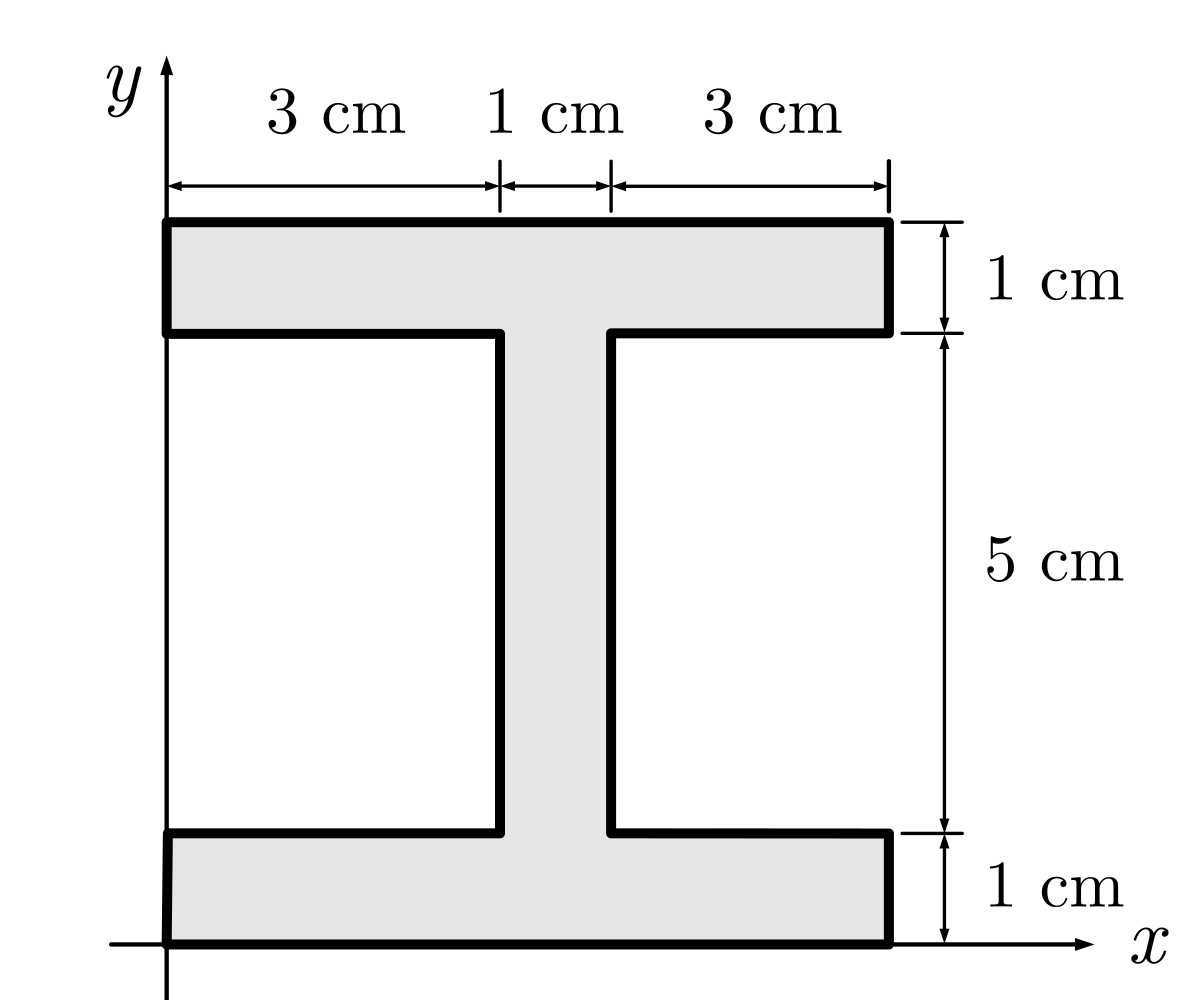
\includegraphics[width=0.5\textwidth,height=0.5\textheight,keepaspectratio]{fig.png}
\end{figure}


